\documentclass{BrJG_submit}
\usepackage{comment}
%%%%%%%%%%%%%%%%%%%%
%
% 
\title{Updated assessment of ${\Delta^{14}CO_{2}}$ measurement intercomparability using atmospheric records and standard materials}
% \shorttitle{Short title goes here}

%%%%%%%%%%%%%%%%%%%%
%    Keywords: list 3 to 5 relevant keywords to the manuscript, separate them by semicolon. Avoid repeating 
%    words in the title. Use lower case. Capital letters only when spelling requires.
% \keywords{keyword 1; keyword 2; keyword 3; keyword 4; keyword 5}
%
\begin{document}


\begin{abstract}
The abstract should describe your research in approximately {\bf 300 words}. These parts should not include references, figures or tables. A well-written abstract can help readers understand the essence of your manuscript and, sometimes, decide whether to continue reading it. We suggest authors to follow briefly the structure of the manuscript in the abstract, including Introduction, Methods, Results and Conclusions. The text should be clear and objective, faithfully representing the subject.
\end{abstract}


\section*{INTRODUCTION}

The first paragraph in a section (without indentation): The Brazilian Journal of Geophysics–BrJG is a quarterly journal of the Brazilian Geophysical Society (SBGf), with arbitration and open access, devoted to the national and international dissemination of original scientific and technical articles related to research in geophysics and geophysical applications in the areas of Geological Sciences, Oceanography, Atmospheric Sciences, and Space Sciences.

New paragraph (with indentation): use this style when you need to begin a new paragraph.
The sections headings are positioned to the left margin (without indentation) in boldface type. The main sections have headings written in all capital letters. Do not number sections of the text. Refer to sections by name.

The body of the manuscript should be written in one column with 1.5 spacing, using Arial font size 11, justified and presenting top, bottom and left margins of 2 cm and a 1.5 cm right margin.

The INTRODUCTION is a mandatory section. So, you have an opportunity to write here a good and brief introduction in a context and background that clearly define the purpose of the study. The references included in the Introduction must be presented to discuss previous and current research in the area and to strengthen the importance of your argument. Don’t forget to present the problem studied, the questions to be answered and the research approach. Highlight the main conclusions, leading the reader to clearly understand the motivation of your research.
\newpage
\section*{METHODS}
The following institutions' radiocarbon measurements (${\Delta^{14}C}$ and/or FM) 
 were compared with the GNS Rafter Radiocarbon Laboratory in turn, each elaborated upon in the following sections. Each intercomparison is tailored specifically to the type of data available between each institution. 

\subsection{Rafter Radiocarbon Lab}

The rafter lab operates the longest runnnig record of atmospheric 14CO2...

\subsection{Heidelberg University}
\subsubsection{Available Data}

The Heidelberg University Institute of Environmental Physics in affiliation with the ICOS Central Radiocarbon Laboratory operates a network of time-series stations measuring ${\Delta^{14}CO_{2}}$. One of these stations, Cape Grim, Tasmania (CGO; 40.68S, 144.68E, 94 m a.s.l; Levin et al., 2010), is a reasonable candidate through which to compare Heidelberg University to Rafter Radiocarbon Lab ${\Delta^{14}CO_{2}}$. Cape Grim and Baring Head observe a similar mixture of air from the Southern Ocean and Austrailia (Ziehn et al., 2014, Law et al, 2010), and a short initial time-series indicates no measurable differnece between the sites from 2017-2019 (~\ref{fig:bhdvcgo}). 
What method was used for sampling? (NaOH)


While the BHD record extends from 1950 to the present, the CGO record includes available data from 1987 to 2016, resulting in 30 years of overlapping data for intercomparison. 
Two intervals will are ignored: 1995-2006 and 2009-2012.
Variability in BHD exists between 1995 and 2005 as 1) the Rafter measurement method was changed from gas counting to AMS and 2) an online $^{13}C$ measurement allowed for approporiate fractionation correction (Turnbull et al, 2017; Zondervan et al., 2015), therefore this interval is ignored in the intercomparison. 
Additionally, the interval of 2009-2012 is ignored as the BHD record sees increasing noise in this period related to a temporary change in NaOH sampling protocol. Further details on the decision to remove these data can be found in the Supplementary Information. 
The remaining overlapping intervals are parsed into 4 sections: 1987 - 1991; 1991 - 1994; 2006 - 2009; 2012 - 2016. 
Each of these data intervals are non-stationary time-series containing seasonality. 

\begin{figure}[h!]
  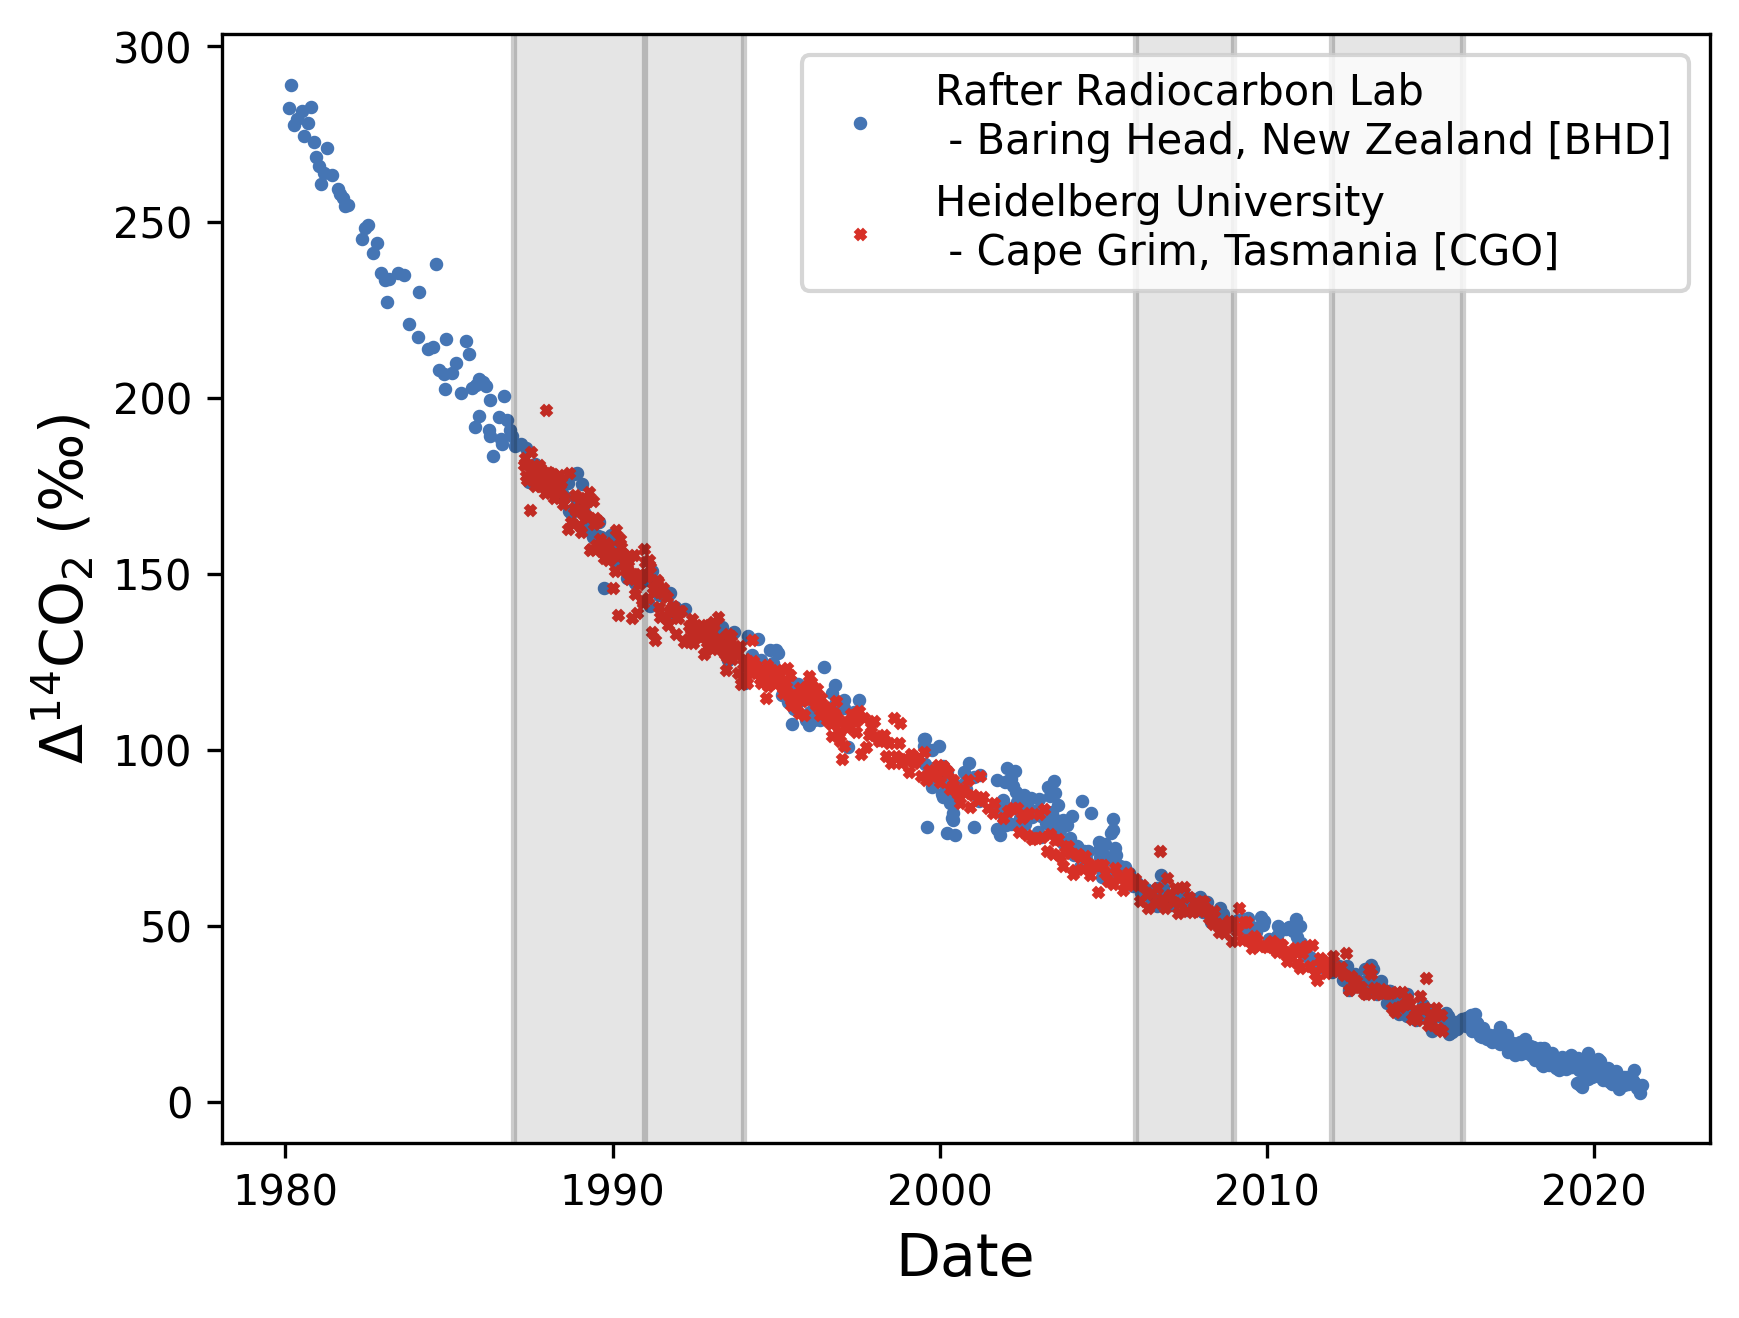
\includegraphics[width=1\textwidth]{new_test.png}
  \caption{Visual summary of available data used for intercomparison between Heidelberg University and Rafter Radiocarbon Lab. The four time intervals of focus are highlighted with background grey: 1987 - 1991, 1991 - 1994, 2006 - 2009, 2012 - 2016 }
  \label{fig:results1}
\end{figure}



\subsubsection{Curve Smoothing}
To extract long-term systematic offsets between institutions, and remove seasonality, the CCGCRV curve fitting procedure (Thoning et al., 1989; www.esrl.noaa.gov/gmd/ccgg/mbl/crvfit/) is implemented similar to (Turnbull et al., 2017). We employ the "smooth" and "trend" functions of the CCGCRV algorithm. "Smoothed" data includes the results of the polynomial and harmonic fits of the data, and a long-term low-pass filter of 667 days. "Trended" data is similar; but retains the polynomial fit to the function and ignores harmonic components. 
Since the BHD and CGO data were not sampled on the same dates (i.e., they have an unequal number and value of x-components which impairs direct comparison of fitted data), the CCGCRV algorithm is programmed to output each smoothed/trended curve in 348 equal steps from 1987 to 2016 (12 samples/year), slightly underestimating the average sampling resolution of each dataset (CGO: 17 samples/year; BHD: 12.25 samples/year). By controlling the x-values of smoothed/trended data output from CCGCRV, the datasets can be compared. 
Error-estimates from the curve smoothing processes are obtained via a Monte-Carlo simulation, run to 10,000 iterations. 

The following process occurs during each iteration for both BHD and CGO data: 
\begin{itemize}
	\item For each x-value, the y-value is  randomly re-assigned, weighted about its normal distribution (1-${\sigma}$ error). 
	\item This randomized time-series is smoothed/trended with CCGCRV algorithm 
	\item The generated data (in 348 equal steps from 1987 to 2016) is appended to a growing dataframe of smoothed/trended data.
\end{itemize}
When the loop is complete, the mean and standard deviation of y each 348 x-values is calculated for BHD and CGO. These computed values are used to assess the intercomparability of BHD and CGO, and thus, Rafter Radiocarbon Lab and Heidelberg University over time. This Monte-Carlo simulation is shown on a small scale in Figure \ref{montecarloexplained}. Statistics are then computed for each of the four time-intervals described above. 

\begin{figure*}[!t]								%[tbhp]
\centering
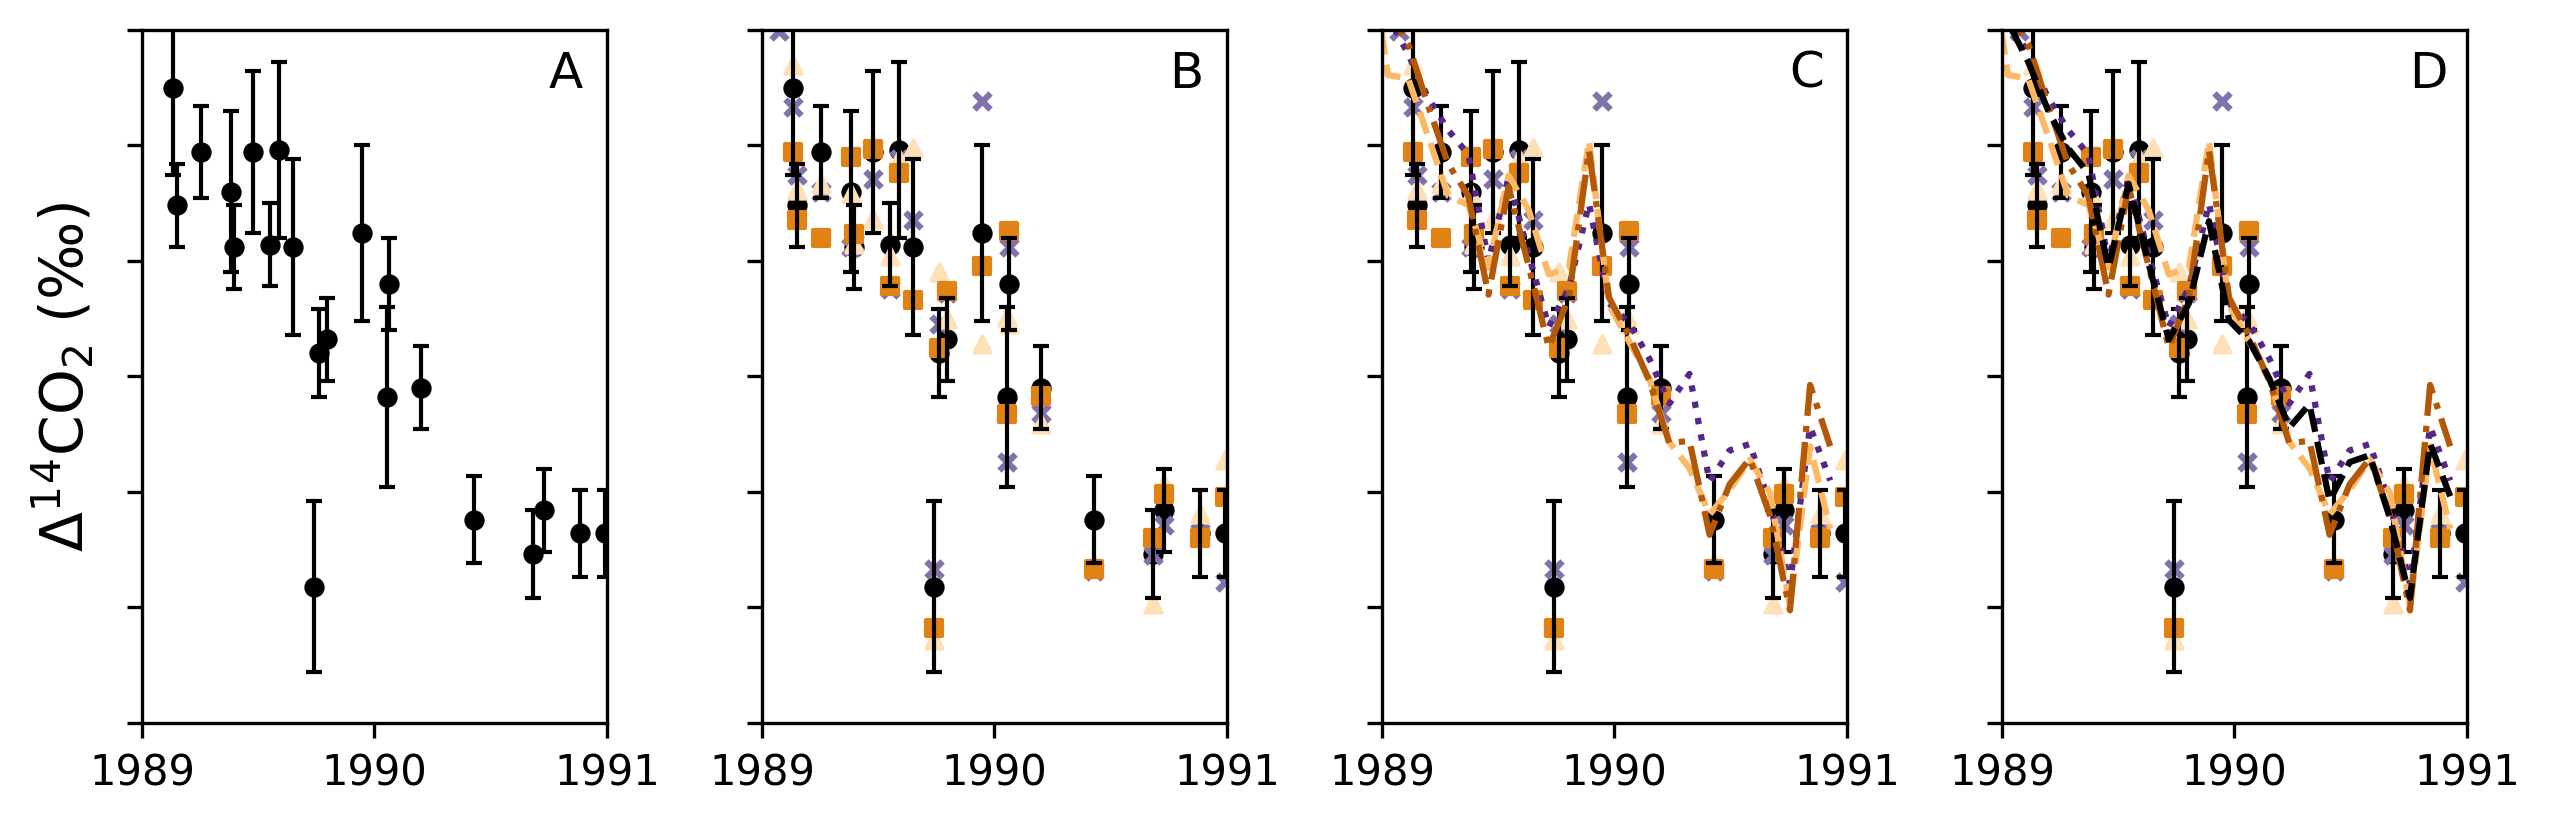
\includegraphics[width=\textwidth]{DEV_FirstDraft_figureS1.png} % inside { } should be the path to the image file
\caption{Visualization of the Monte Carlo simulation to generate an uncertainty estimate about the CCGCRV curve smoothing algorithm.}	% Include the figure caption here
\label{fig:montecarloexplained}									% Include a unique label here, so you can refer to the figure
\end{figure*}


\begin{itemize}
	\item Need to add details about NaOH sampling method. 
\end{itemize}

\begin{itemize}
	\item Need to add details about NaOH sampling method. 
\end{itemize}


\subsection{Scripps Institude of Oceaography / Lawrence Livermore National Laboratory}

RRL and Scripps Institude of Oceaography / Lawrence Livermore National Laboratory (SIO/LLNL) are compared through measurement of the same standard materials: Niwot Ridge 3 and Niwot Ridge 4 (NWT3 and NWT4). NWT3 and NWT4 are air standards from Niwot Ridge, Colorado collected in 2005 and 2006, the latter "spiked" with fossil ${CO_{2}}$. In these particular measurements, standards were graphitized and combusted at SIO and ${\Delta^{14}C}$ measured at LLNL. This intercomparison is sparse in terms of temporal overlap, with RRL measurements ranging from 2013 to 2020; and LLNL measurements encompassing March - April 2009. 
\subsection{Australian Nuclear Science and Technology Organisation (ANSTO)}

Intercomparability between ANSTO Centre for Accelerator Science and RRL ${\Delta^{14}C}$ is assesed via measurements of Kauri tree-rings. Both Institutions measured the same samples in this intercomparison.   
\begin{itemize}
	\item How was the sample prepared? Other details to add. 
\end{itemize}

\subsection{University of Magallanes (DO NOT PUBLISH WITHOUT EXPRESS PERMISSION FROM RICARDO}
  
Intercomparability between University of Magallanes and RRL ${\Delta^{14}C}$ is assesed via measurements of tree-rings in Monte Tarn, Chile (53S. Samples from either institution were collected from the same site; but not the same tree. 
\begin{itemize}
	\item How was the sample prepared? Other details to add. 
\end{itemize}


\subsection{Statistical Analyses}
For intercomparisons of non-stationary time-series, such as RRL vs ANSTO, University of Magallanes, and Heidelberg University, intercomparability is assessed using paired (relative) t-tests. Comparison with SIO/LLNL uses an independent t-test. In all cases, the null hypothesis is that no difference between the institutions exists. The hypothesis is rejected if p-values are <0.01 (these are displayed in Table X). Statistical calculations were made using the Python scipy.stats library (https://docs.scipy.org/doc/scipy/reference/stats.html).



%
%
%
%
\newpage
\section{Results}

\subsection{RRL vs. Heidelberg University}

\begin{itemize}
	\item remind the reader what the values are: (as I need to remind myself), the values shown here are the means of each output x value from my controlled x-outputs
	\item the values in the table are the means and standard deviations on the offsets within each time period
	\item Describe the offsets between BHD and CGO for each time period, and if there is any difference between the trend and smooth curves? 
	\item Talk a little bit about the differences between BHD and CGO develop over time, and this will be elaborated further in the dsicussion
\end{itemize}













































\begin{figure}[h!]
  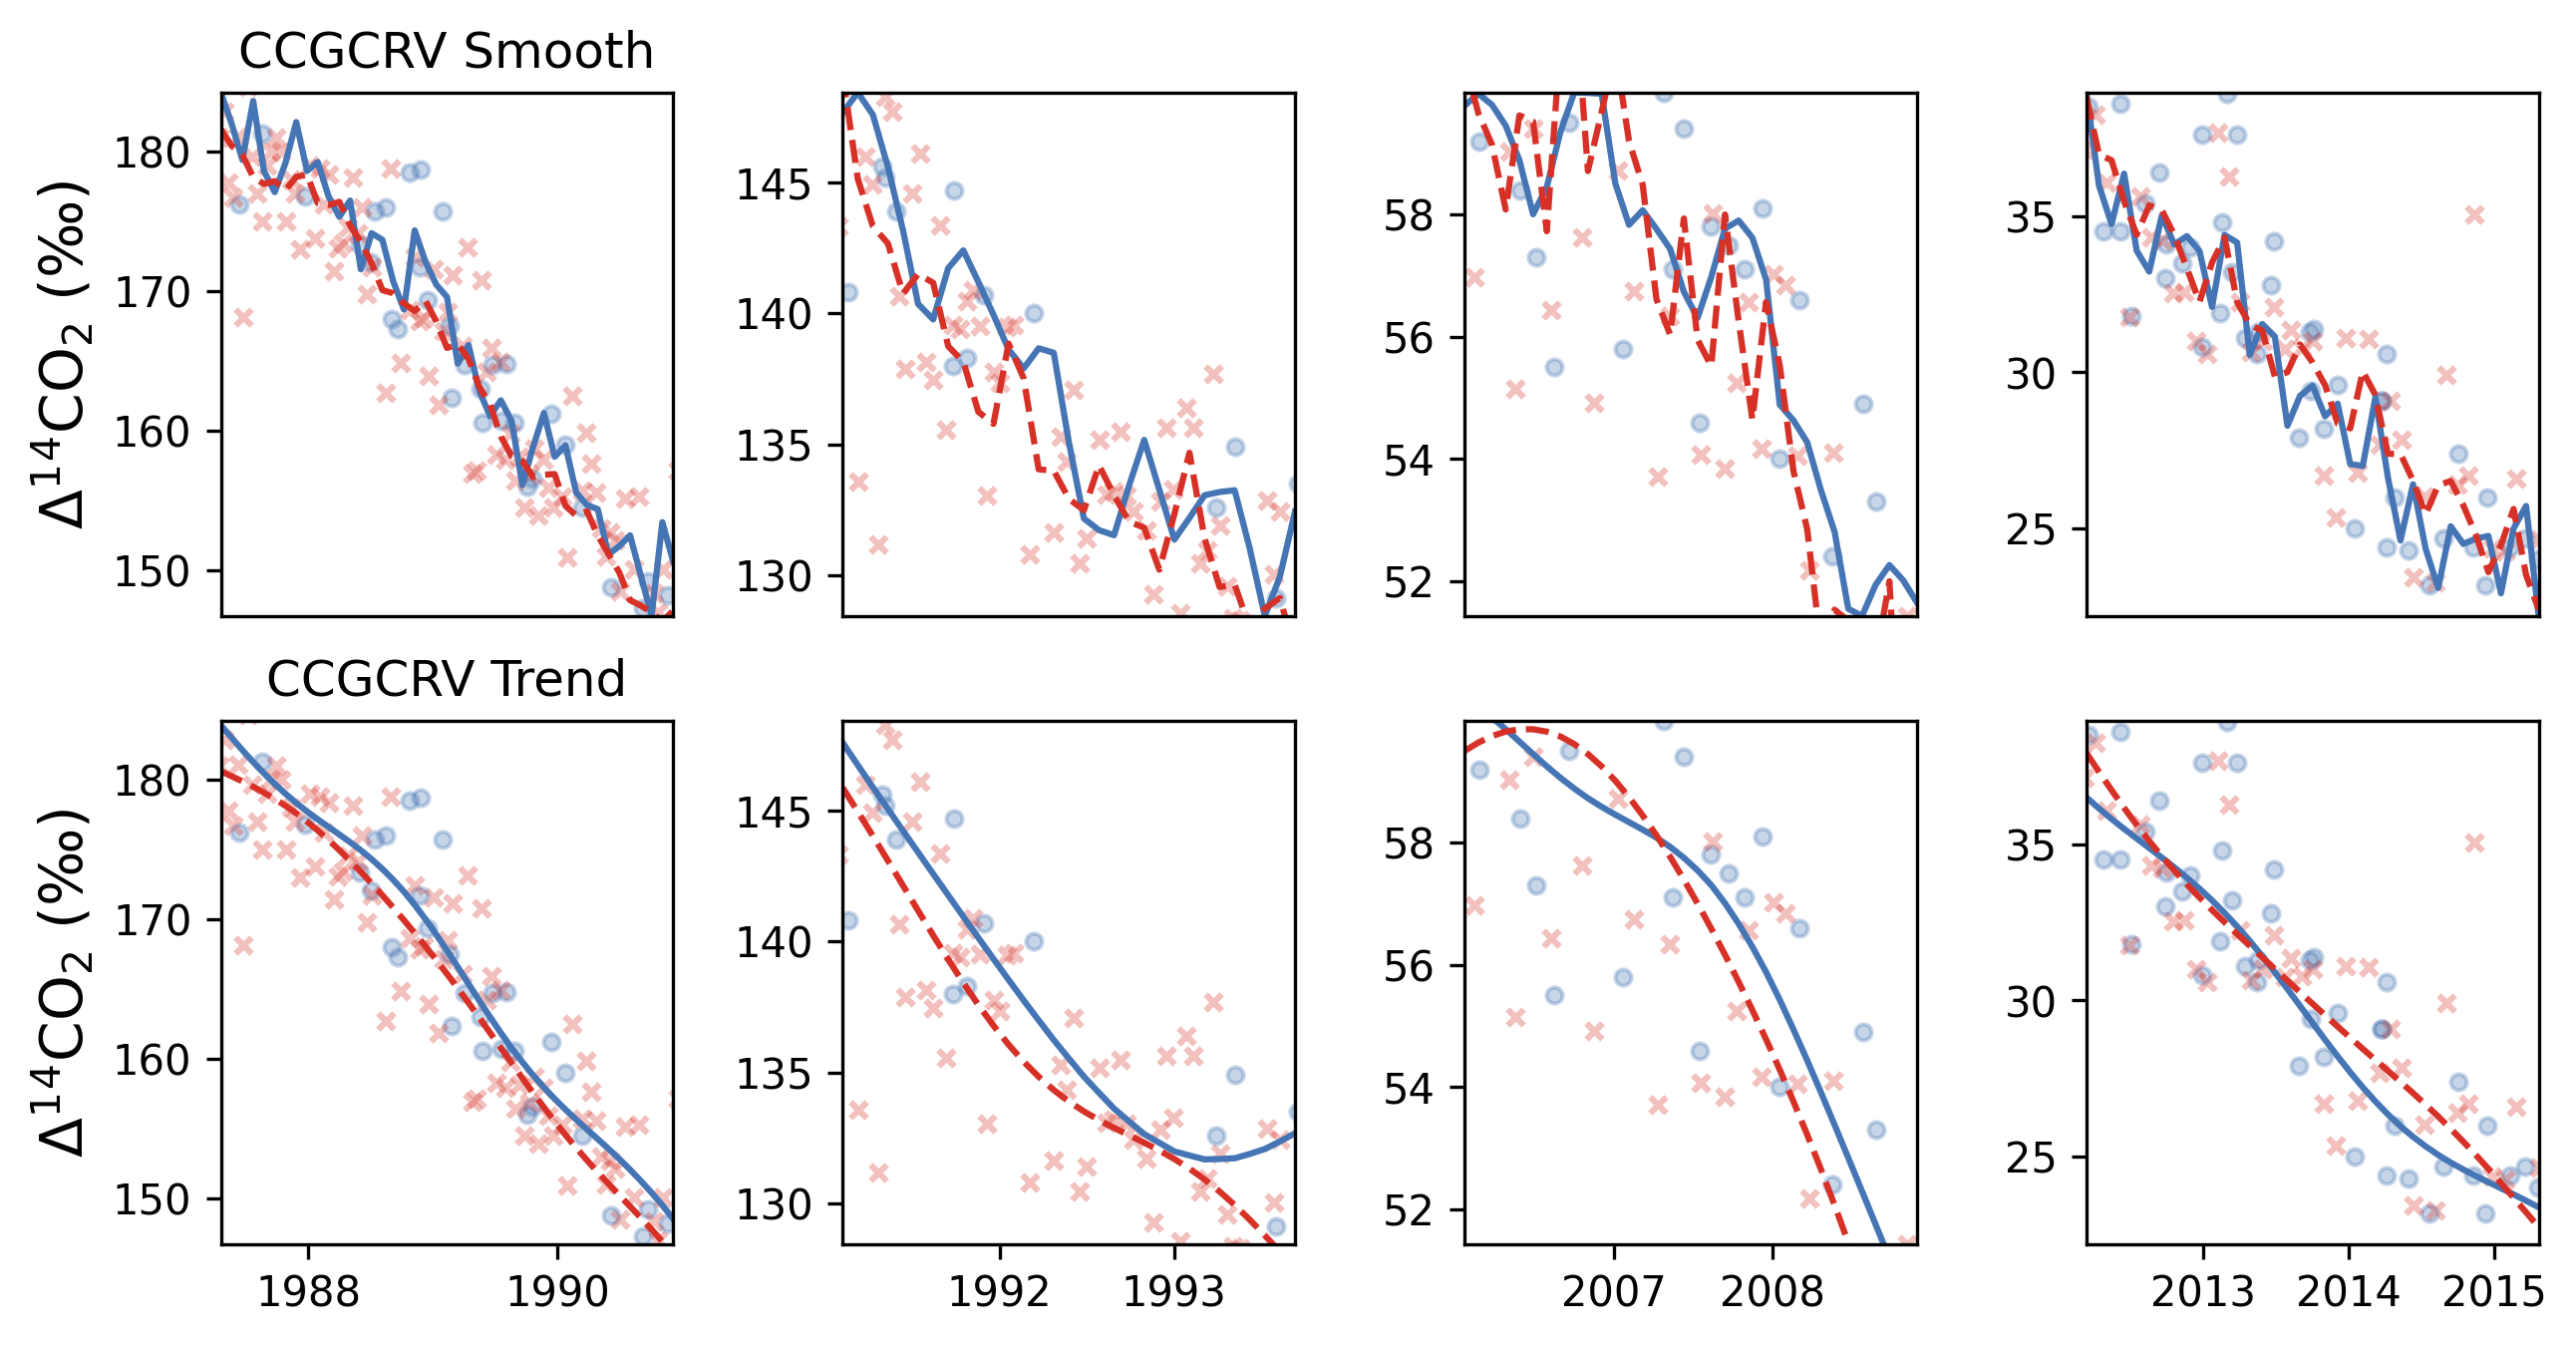
\includegraphics[width=1\textwidth]{DEV_FirstDraft_figure3b_D14C.png}
  \caption{Means of Monte Carlo simulation using CCGCRV "smooth" function (top panel), and "trend" function (bottom panel) overlaid upon initial CGO and BHD data. Panel a-d represents the various time-intervals used in this intercomparison: 1987 - 1991, 1991 - 1994, 2006 - 2009, 2012 - 2016}
  \label{fig:results1}
\end{figure}


\newpage
\subsection{ANSTO and University of Magallanes}
\begin{figure}[h!]
  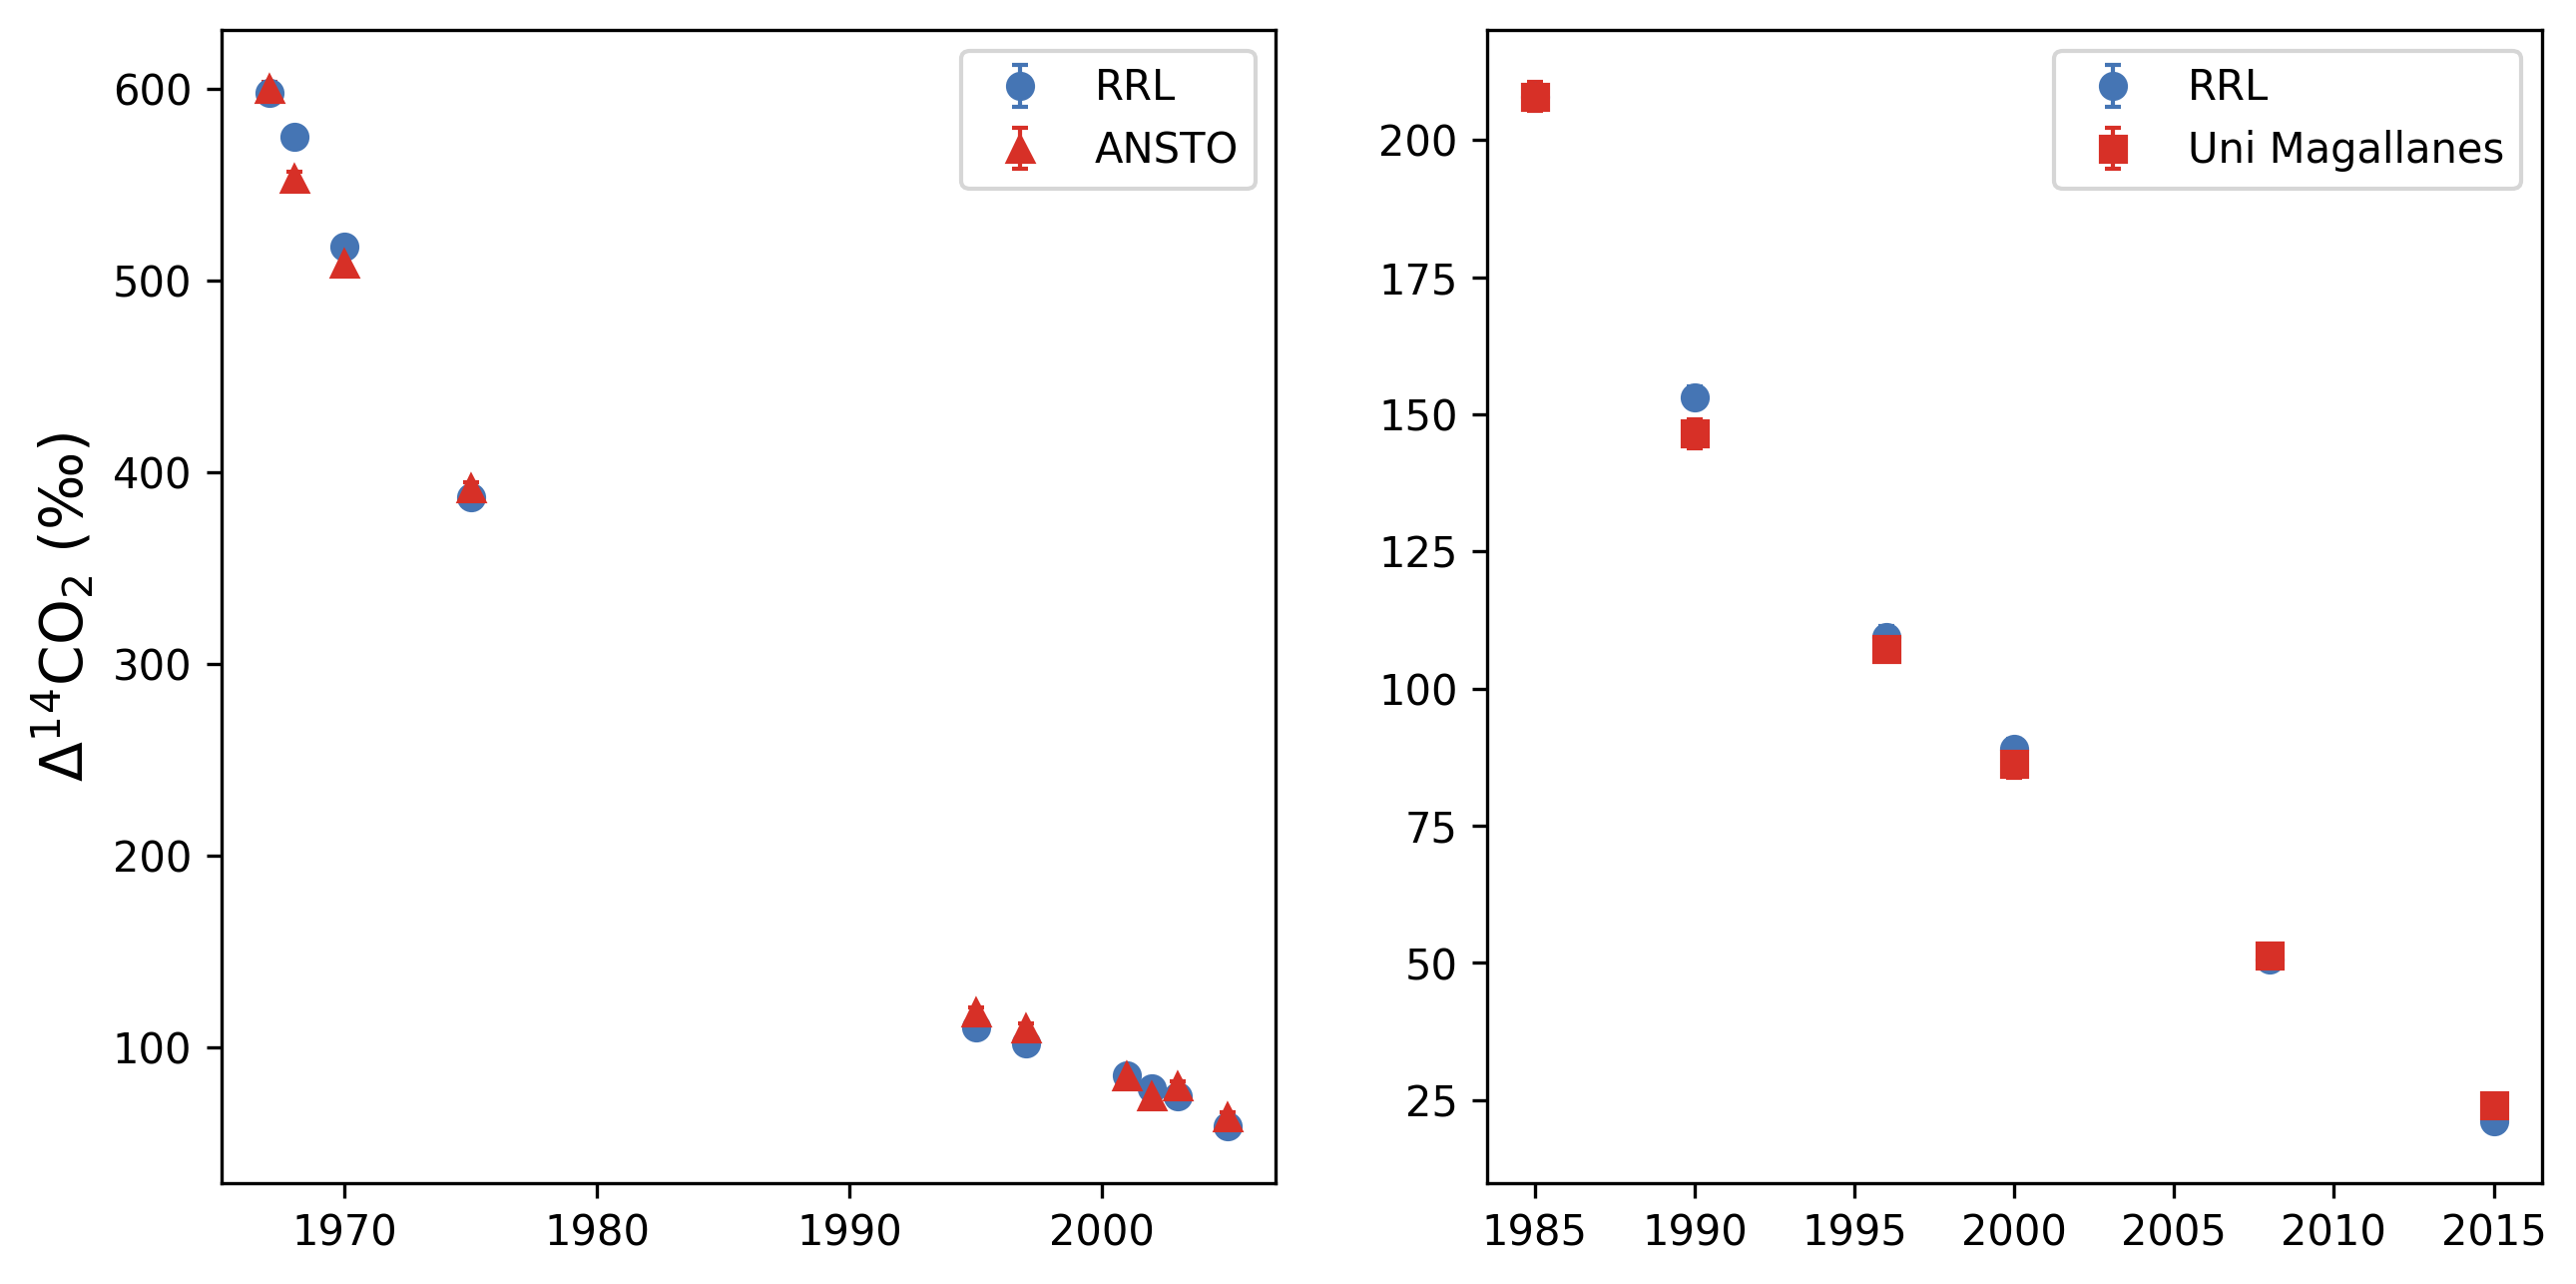
\includegraphics[width=1\textwidth]{Magallanes_Ansto_comb.png}
  \caption{ADD CAPTION LATER}
  \label{fig:results1}
\end{figure}

\newpage
\subsection{SIO / LLNL}

\begin{figure}[h!]
  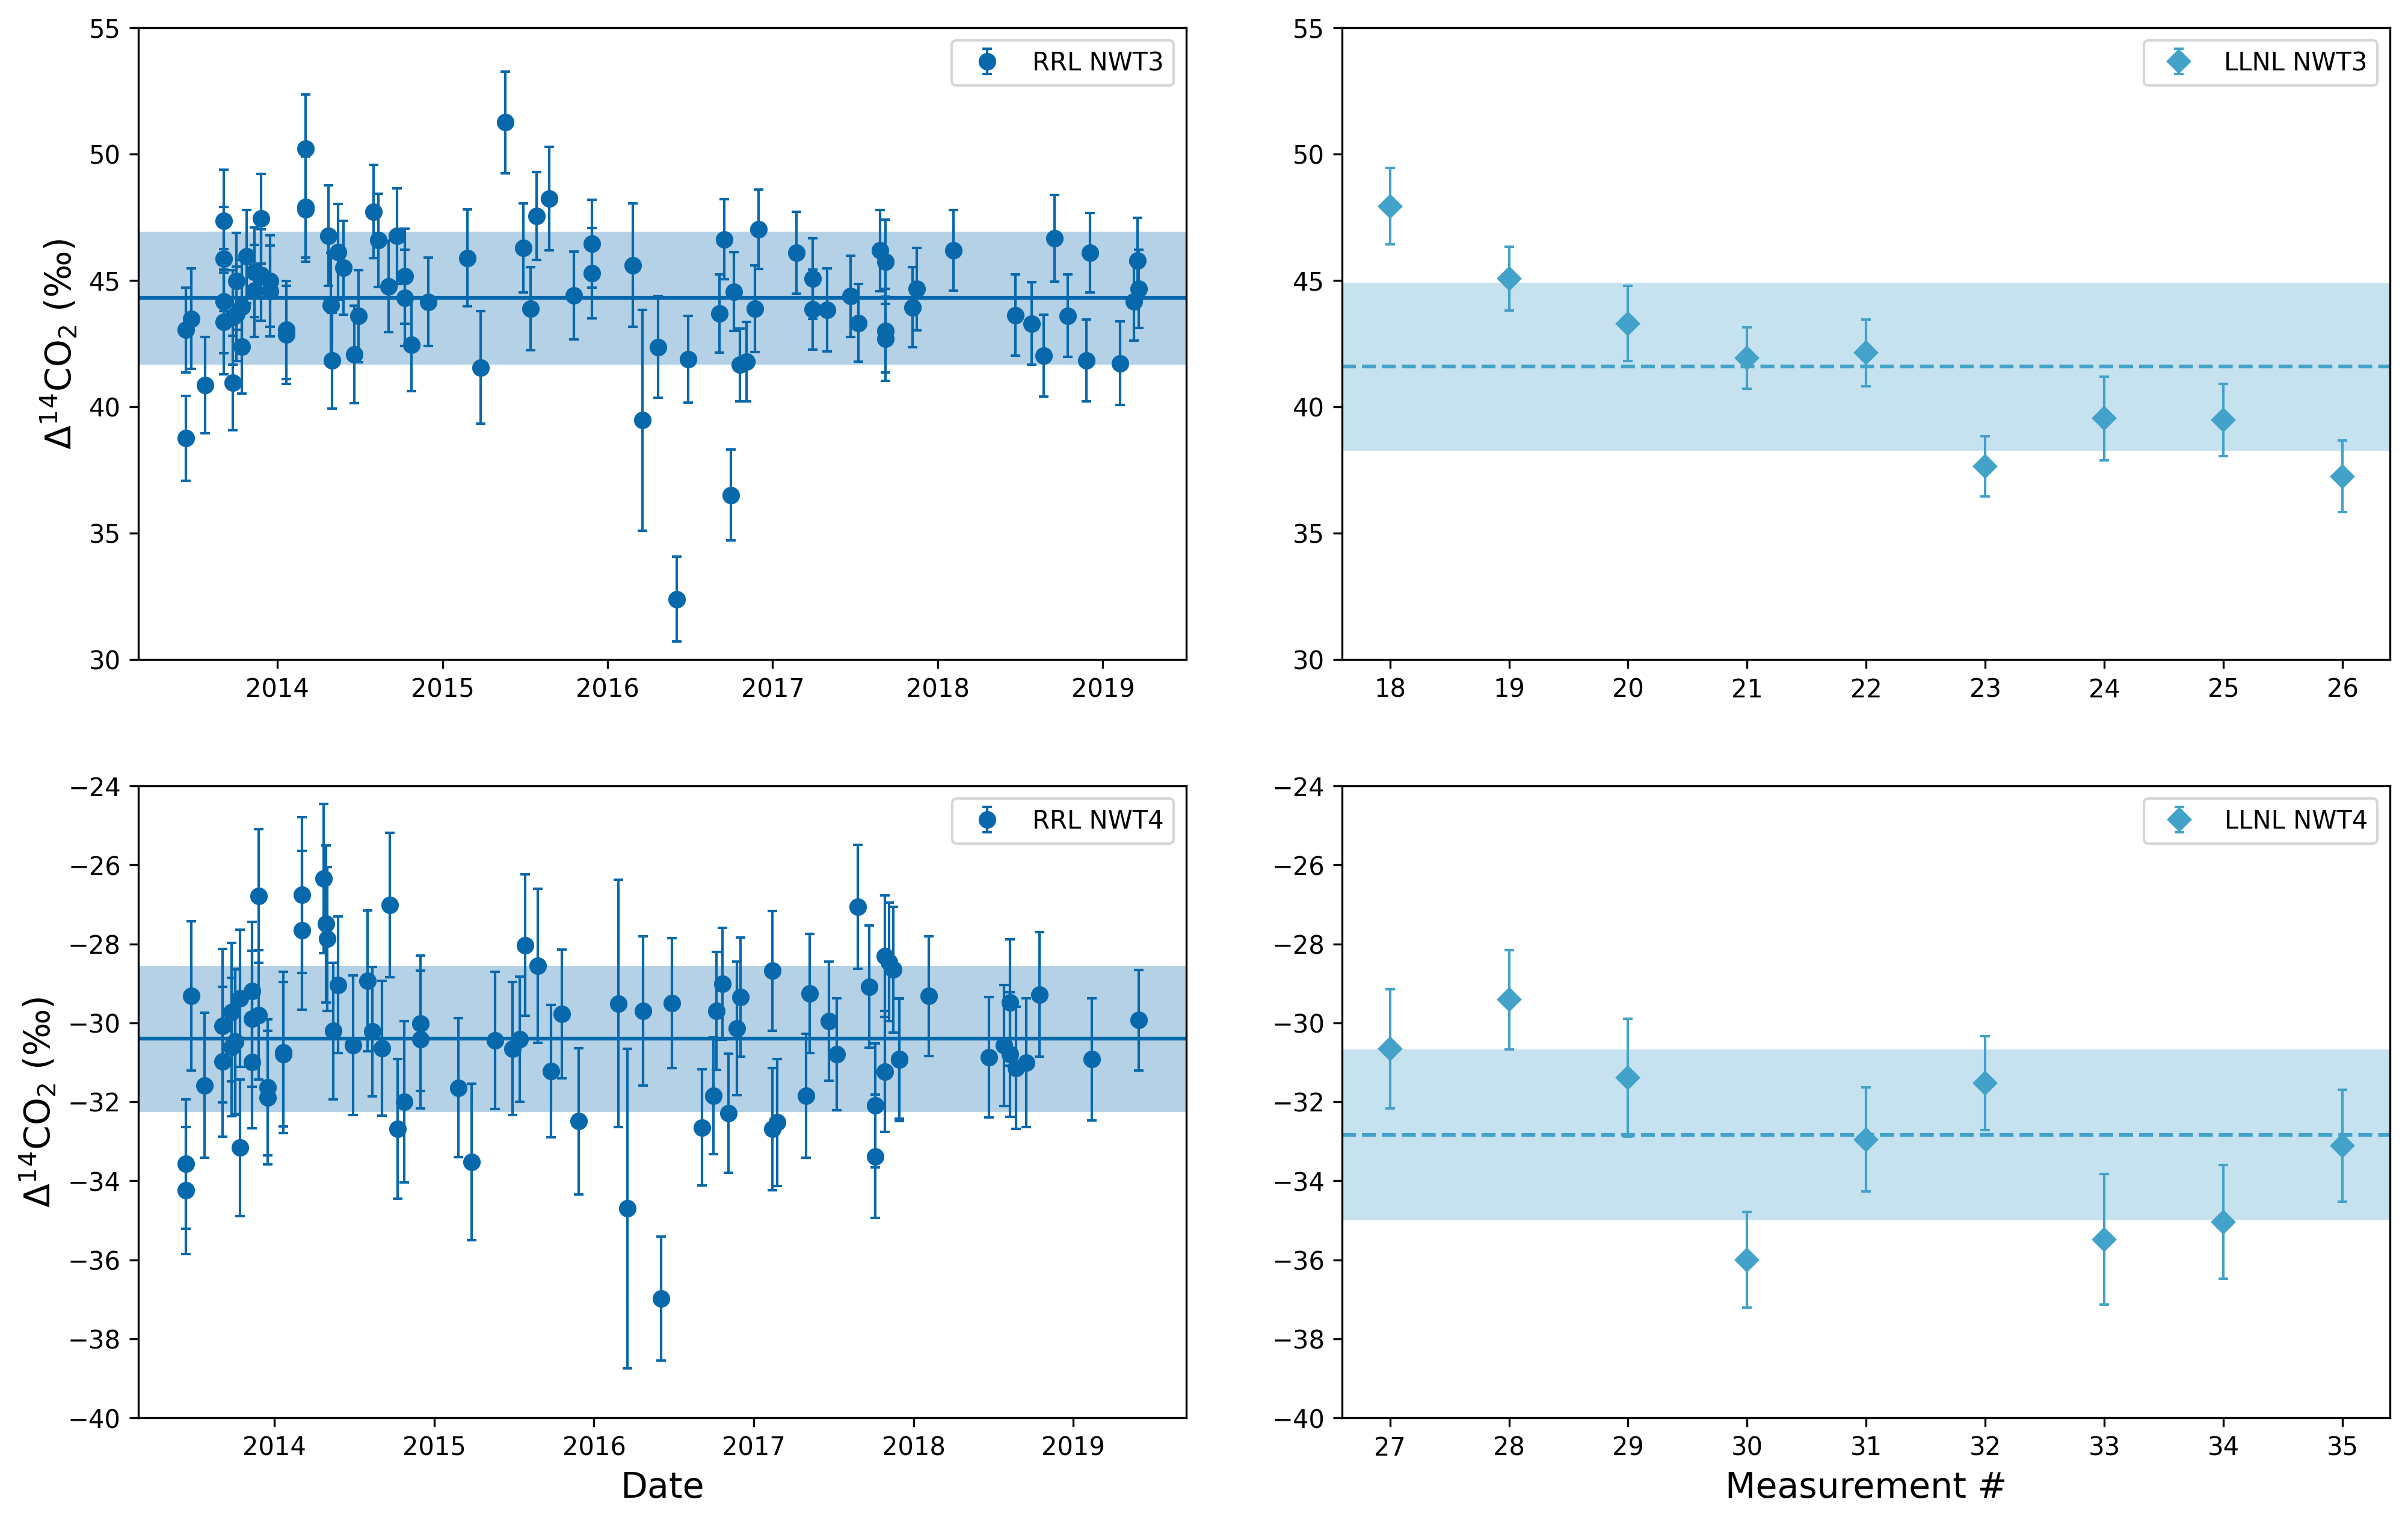
\includegraphics[width=1\textwidth]{SIOLLNLvRRL.png}
  \caption{Top panel shows ${\Delta^{14}CO_{2}}$ measurements of NWT3 standard from RRL (a) and SIO/LLNL (b), respectively. Bottom panel similarly shows NWT4 standard.}
  \label{fig:results1}
\end{figure}

\newpage
\begin{tabular}{ |p{7.5cm}||p{4cm}|p{1.5cm}|p{2.5cm}| }
 \hline
 \multicolumn{4}{|c|}{Result Summary } \\
 \hline
 Institute vs. RRL       &  ${\Delta\Delta^{14}C}$ &  p-value & Result\\
 \hline
Heidelberg [1987 - 1991] (Smooth/Trend) & 1.85\pm0.30,      1.87\pm0.30          &  $3.0x10^{-7}$  & Different \\
Heidelberg [1987 - 1991] (Smooth/Trend) & 1.90\pm0.43,       1.73\pm0.43                 & $4.0x10^{-4}$ & Different  \\
Heidelberg [1987 - 1991] (Smooth/Trend) & 0.55\pm0.22,       0.58\pm0.26                  & 0.03 & NOT different \\      
Heidelberg [1987 - 1991] (Smooth/Trend) & -0.52\pm0.26,       -0.54\pm0.21                    & 0.02  & NOT different  \\
SIO/LLNL(NWT3)          & 2.72\pm1.14 & 0.005   & Different  \\
SIO/LLNL(NWT4)           & 2.44\pm0.75 &  $4x10^{-4}$          & Different  \\
ANSTO                    & 0.46\pm2.76 & 0.878  & NOT different \\
 \hline
\end{tabular}














































\newpage
\section*{DISCUSSION}
I think this section will be a little short
\begin{itemize}
	\item Begin by describing what is controlling the variability in the offset between BHD and CGO. This is strongly linked to our change in instrumentation / usnig XCAMS, and the additino of online 13C correctino.
	\item The importnace of this is: the dataset with the longest record reveals the potential variability in two institutions over time; wrt to instruments, users, and associated combustion/graphitization blanks that can all lead to small but persistent offsets that may propogate through the science. This Heidelberg intercomparison shows that in order to get meaningful understandings of the true intercomparability of institutions over time, it must be constantly repeated. 
	\item this is somethign we will address in upcoming iterations of intercomparison, similar to Miller et al., 2013. 

\end{itemize}



\section*{CONCLUSION}
This section is mandatory.

As a suggestion, this section may include (1) principles, relationships, and generalizations inferred from the results (but not a restatement or summary of the results); (2) any exceptions to or problems with those principles, relationships, and generalizations, as indicated by the results; (3) agreements or disagreements with previously published work; and (4) implications and significance of the work.

The conclusion should not include figures, tables, equations, or reference citations.


\section{Supplementary Information}
\label{sec:conc}




\subsection{Site Intercomparison of Baring Head and Cape Grim}
\begin{figure}[h!]
  \caption{ Intercomparison of ${\Delta^{14}CO_{2}}$ measurements  at Cape Grim, Tasmania (CGO), and Baring Head, New Zealand (BHD) collected by NIWA and measured at Rafter Radiocarbon Laboratory. Dates represent the middle of the sampling period, which differ no more than one day between sites. These data show that during the time in which data are available, no measureable difference is found between the two sites. This provides some evidence that the two sites may be considered equivalent for this intercomparability study.}
% This data originally was sent to me in Jocelyn's first dropbox file. Later it was condensed to the currnent file in the H: drive.  H:\Science\Datasets\CGOvBHD
  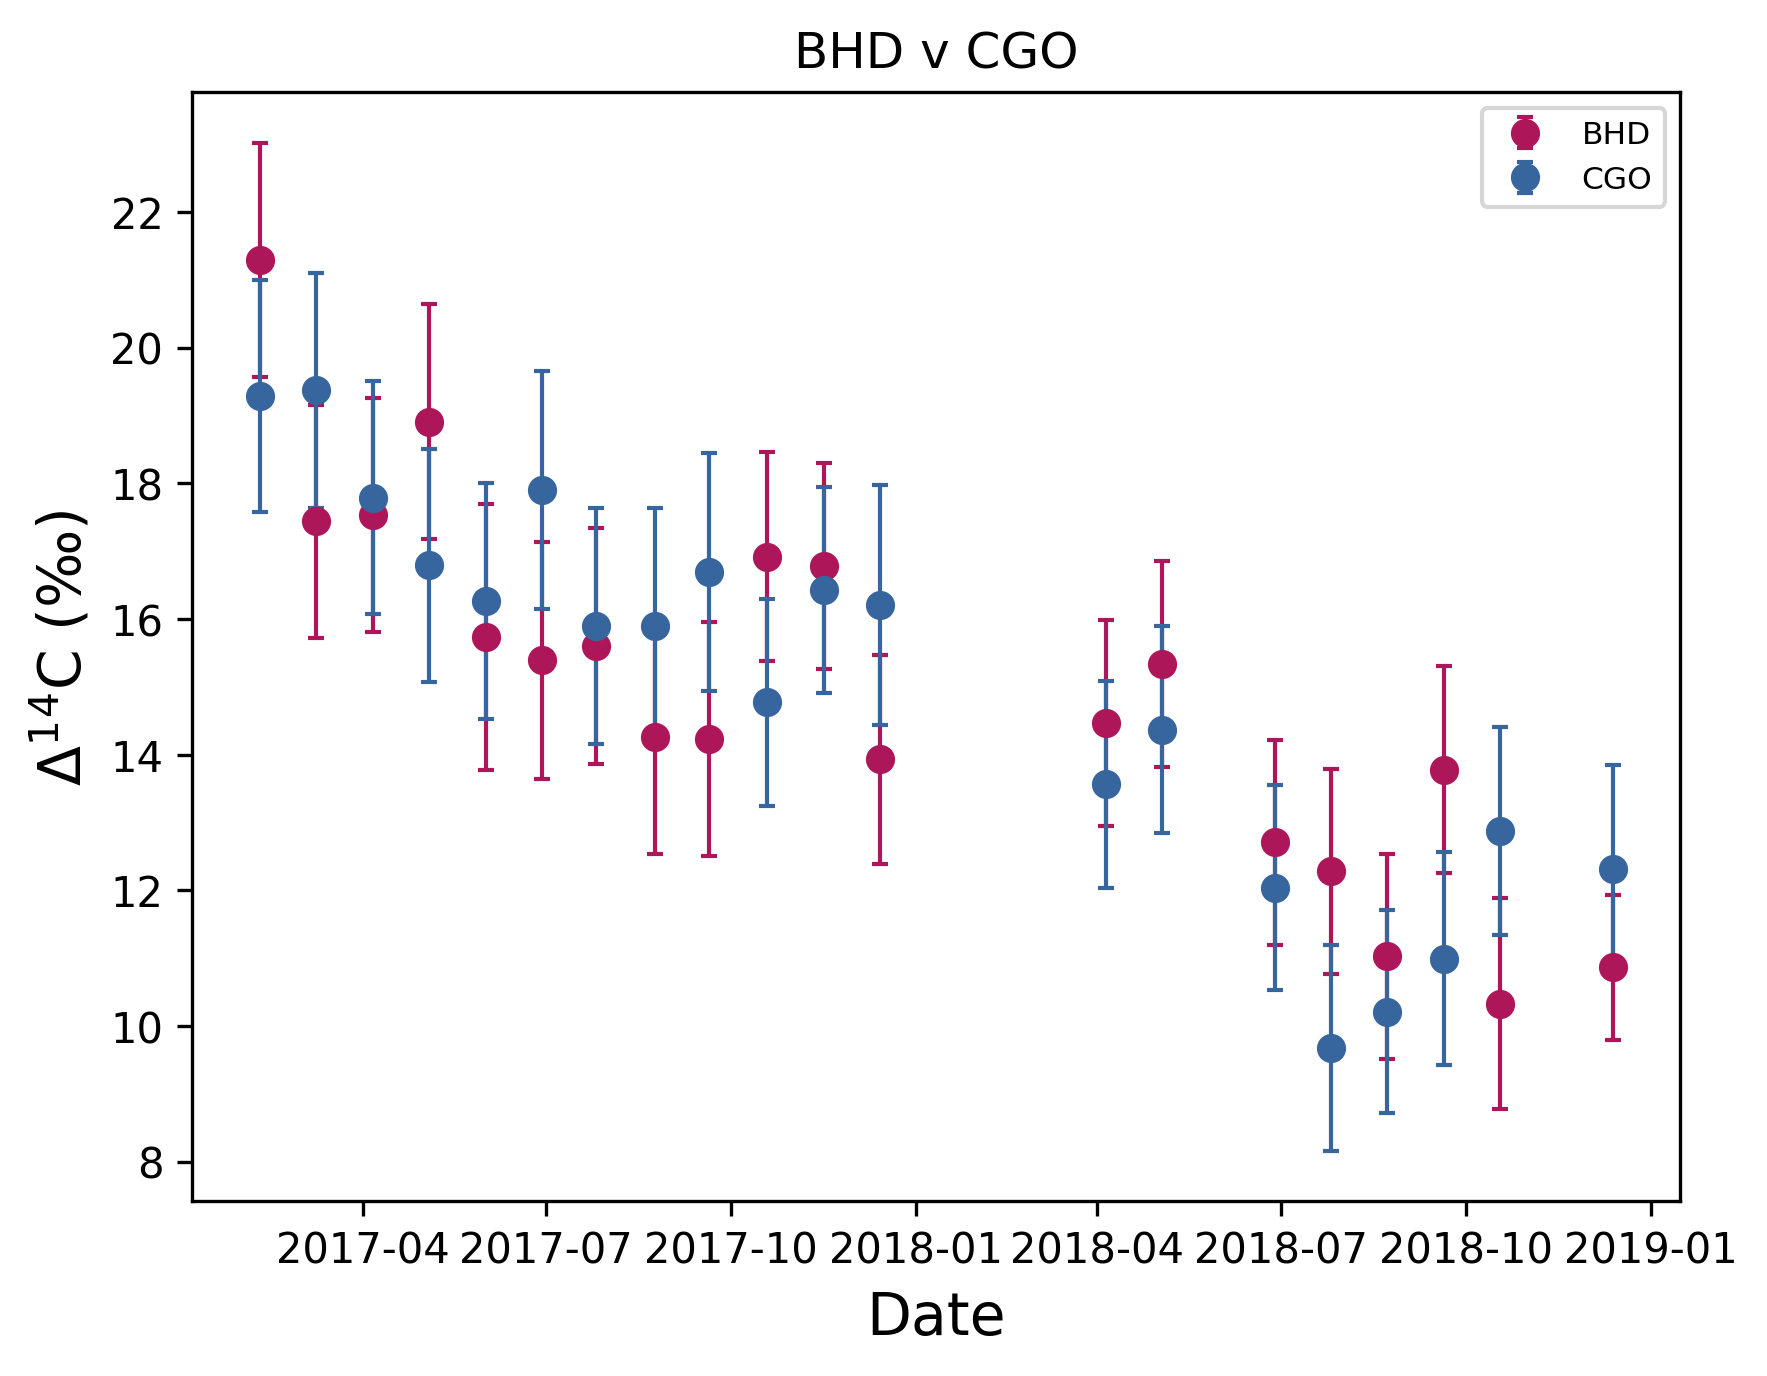
\includegraphics[width=1\textwidth]{Site_intercomparison.png}
\label{fig:bhdvcgo}
\end{figure}

\subsection{Removal of data interval 2009 - 2012 in Rafter vs. Heidelberg University Intercomparison}
















\begin{comment}

\section*{ACKNOWLEDGMENTS}
When necessary, acknowledgments and credits to the funding institutions should appear in the Acknowledgments section. This section is to appear in the published paper and must NOT be included in the submitted manuscript.

\section*{Data and materials availability}
The data used in the manuscript should be open and publicly available whenever possible.

If appropriate, the BrJG encourages authors to archive data in a permanent repository. The data deposited should be cited in the reference list of the manuscript using the DOI or other persistent identifiers.


\appendix

\section{Title of the appendix}
The appendix is an optional section that can include supplementary data and information to the main text. All appendix sections must be cited in the main text. In the appendixes, figures, tables, equations etc. should be labeled starting with ``A'' or ``B'', e.g., Figure A1, Equation A1, etc. 
\begin{equation}
	a = b
\end{equation}

\section*{Reference formating}
Papers published in BrJG follows guidelines set forth in The Chicago Manual of Style, 17th edition. The references are listed in alphabetical order of first author’s surname and not numbered. When several references of the same first author appear, a single-author work precedes a multiauthor work. References with identical authorship should be listed in chronological order.

References can provide greater credibility to the article, when properly chosen. The current state of the research field should be reviewed carefully and key publications cited. Priority should be given to citation of updated references, published in the last five years, considering the period of manuscript submission.

The abbreviations of the journals names can be found in the database in which the journal is indexed or in the World List of Scientific Periodicals. Include the digital object identifier (DOI) for all references where available.

{\bf In the text, citations should be consistent with those in the reference list and vice versa}. References will be cited as: \cite{OLIOSO1999341}; \cite{LEGCHENKO20023};  \cite{bott13}; or  \citep{OLIOSO1999341,LEGCHENKO20023,bott13}, for example. Articles by the same authors and presenting the same dates must be distinguished, with a lowercase letter (a, b, c...) after the year. References must be arranged in alphabetical order in the text (including citations in tables and legends) and listed individually at the end of the manuscript.

Authors are requested to avoid references to proceedings of conferences. It is appropriate only if these proceedings are available to the reader.

\section*{AUTHOR CONTRIBUTIONS}
It is expected that each author has made substantial contributions to the work, at least two criteria are considered for authorship: actively participate in the discussion of results; and revise and approve the final version of the manuscript. In this section, at the end of the article, the individual contribution should be clearly stated:\\ {\bf 1st Author}:… {\bf 2nd Author}:… {\bf 3rd Author}:…

\section*{Conflicts of Interest}
The authors declare no conflict of interest. The conflict may be personal, commercial, political, academic or financial. If necessary, authors may request that the manuscript not be assessed at certain institutions or reviewers, in order to avoid possible conflicts of scientific interest. 

\section*{Copyright and Open Access}
All copyrights are reserved to authors. The journal keeps the publishing rights.

Ideas, concepts, content and writing style are the sole responsibility of the authors. However, political, commercial or religious quotes will not be allowed in the article.

The BrJG is an open access journal. All articles are published under Creative Commons CC-BY license which means that all content is freely available without charge. Users are allowed to read, download, copy, distribute, print, search, link to the full texts or use figures, maps and other illustrations, when due reference to the article is assigned.

%\newline
This document only illustrates the frequently encountered style elements. Authors should consult the full Instructions to Authors at https://sbgf.org.br/revista/index.php/rbgf/information/authors.

%%%%%%%%%%%%%%
%\newpage

\bibliographystyle{seg}
\bibliography{refs_exemplo}




\end{comment}



\end{document}